% !TEX root = main.tex

\section{贝叶斯决策论} % 2.1-2.9 (2.10-2.11)
% 贝叶斯判定
% 正态分布的判别函数
% 样本均值 协方差矩阵
% 连续特征 离散特征 x\in\{0,1\}

\subsection{离散变量}
处于类别$\omega_i$并具有特征值$x$,有后验概率\footnote{通常用$p(\cdot)$代表概率密度函数(连续变量),用$\pr{\cdot}$代表概率质量函数(离散变量)}\textemph{(给特征判类别)}
\[\prc{\omega_i}{x}=\frac{p(x\mid\omega_i)\pr{\omega_i}}{p(x)}\]
即
\[posterior=\frac{likelihood\times prior}{evidence}\]

无论什么情况,当我们观察到特定的$x$,对于二分类问题有错误率
\[\prc{error}{x}=
\begin{cases}
\prc{\omega_1}{x} & \text{决策}\omega_2\\
\prc{\omega_2}{x} & \text{决策}\omega_1
\end{cases}
=\min[\prc{\omega_1}{x},\prc{\omega_2}{x}]\]
分段函数的分界点成为\emph{决策边界}。

平均错误概率可表示为
\[\pr{error}=\intab{-\infty}{\infty}{\pr{error,x}}=\intab{-\infty}{\infty}{\prc{error}{x}p(x)}\]
注意$p(x)$是证据,可以看为是固定分布(常量)。

\begin{theorem}[贝叶斯决策/最小错误率准则]
若$P(\omega_1\mid x)>P(\omega_2\mid x)$,则判定类别为$\omega_1$;否则判为$\omega_2$。
或有等价判别$P(x\mid \omega_1)p(\omega_1)>P(x\mid\omega_2)p(\omega_2)$。
依照这种准则可以获得最小错误率,即$P(error\mid x)=\min [P(\omega_1\mid x),P(\omega_2\mid x)]$
\end{theorem}

Neyman-Pearson准则是限定某一类别$w_i$的误差率不能超过一个常数,但会导致总的误差率提升。

\subsection{连续变量}
考虑特征向量$\vx\in\rr^d$($\rr^d$称为特征空间),令$\{\omega_1,\ldots,\omega_c\}$表示有限的$c$个类别集,$\{\alpha_1,\ldots,\alpha_a\}$表示有限的$a$种可能采取的行为集,损失函数(loss)$\lambda(\alpha_t\mid\omega_j)$描述类别状态为$\omega_j$时采取行动$\alpha_i$的风险。
$p(\vx\mid\omega_j)$表示在真实类别为$\omega_j$的条件下$\vx$的概率密度函数,$P(\omega_j)$表示类别处于状态$\omega_j$时的先验概率,后验概率$P(\omega_j\mid \vx)$则通过贝叶斯公式
\[P(\omega_j\mid\vx)=\frac{p(\vx\mid\omega_j)P(\omega_j)}{p(\vx)}\]
计算得到,证据变为
\[p(\vx)=\sum_{j=1}^cp(\vx\mid\omega_j)P(\omega_j)\]

与行动$\alpha_i$相关联的风险(risk)为
\[R(\alpha_i\mid\vx)=\sum_{j=1}^c\lambda(\alpha_i\mid\omega_j)\prc{\omega_j}{\vx}\]

进而得到总损失
\[R=\intabu{}{}{R(\alpha(\vx)\mid\vx)p(\vx)}{\vx}\]

因此得到连续情形下的贝叶斯决策论:
\begin{theorem}
为最小化$R$,计算条件概率
\[R(\alpha_i\mid\vx)=\sum_{j=1}^c\lambda(\alpha_i\mid\omega_j)\prc{\omega_j}{\vx},\;\forall i=1,\ldots,a\]
选择$\alpha_i$使得$R(\alpha_i\mid\vx)$最小,进而最小化总的风险即称为贝叶斯风险,记为$R^*$
\end{theorem}

\subsubsection{二类分类}
对称损失/0-1损失
\[\lambda(\alpha_i\mid\omega_j)=
\begin{cases}
0 & i=j\\
1 & i\ne j
\end{cases}
\qquad i,j=1,2,\ldots,c\]
有条件风险
\[\begin{aligned}
R(\alpha_1\mid\vx)&=\lambda_{11}P(\omega_1\mid\vx)+\lambda_{12}P(\omega_2\mid\vx)\\
R(\alpha_2\mid\vx)&=\lambda_{21}P(\omega_1\mid\vx)+\lambda_{22}P(\omega_2\mid\vx)
\end{aligned}\]

可得贝叶斯决策
\[\frac{p(\vx\mid\omega_1)}{p(\vx\mid\omega_2)}>\frac{\lambda_{12}-\lambda_{22}}{\lambda_{21}-\lambda_{11}}\frac{P(\omega_2)}{P(\omega_1)}\]

\subsection{正态密度}
\begin{itemize}
	\item 连续单变量正态函数
\[p(x)=\frac{1}{\sqrt{2\pi}\sigma}\exp\lrs{-\frac{1}{2}\lrp{\frac{x-\mu}{\sigma}}^2}\thicksim N(\mu,\sigma^2)\]
有期望和方差
\[\begin{aligned}
\mu &= \E{x}=\int_{-\infty}^\infty xp(x)\diff x\\
\sigma^2 &=\E{(x-\mu)^2}=\int_{-\infty}^\infty (x-\mu)^2 p(x)\diff x
\end{aligned}\]

	\item $d$维多元高斯分布
\[p(\vx)=\frac{1}{(2\pi)^{d/2}|\Sigma|^{1/2}}\exp\lrp{-\frac{1}{2}(\vx-\vmu)^\T\Sigma^{-1}(\vx-\vmu)}\thicksim N(\vmu,\Sigma)\]
其中$\vmu$为$d$维均值向量,$\Sigma$维$d\times d$协方差矩阵,同时
\[\begin{aligned}
\vmu &=\E{\vx} = \int\vx p(\vx)\diff\vx\\
\Sigma &=\E{(\vx-\vmu)(\vx-\vmu)^\T} = \int(\vx-\vmu)(\vx-\vmu)^\T p(\vx)\diff\vx
\end{aligned}\]
每一元素为
\[\begin{aligned}
\mu_i &= \E{x_i}\\
\sigma_{ij} &= \E{(x_i-\mu_i)(x_j-\mu_j)}
\end{aligned}\]
注意协方差矩阵$\Sigma$通常是对称且半正定的。
但这里我们严格限定$\Sigma$为正定的,使得$\Sigma$的行列式是一个正数。
\end{itemize}

服从正态分布的随机变量的线性组合都是一个正态分布。
特别地,若$p(\vx)\thicksim N(\vmu,\Sigma)$,$A$是$d\times k$的矩阵,且$\vy=A^\T\vx$是一$k$维向量,则
\[p(\vy)\thicksim N(A^\T\vmu,A^\T\Sigma A)\]
协方差用于计算数据沿任何方向或任意子空间的分散程度。
\begin{figure}[H]
\centering
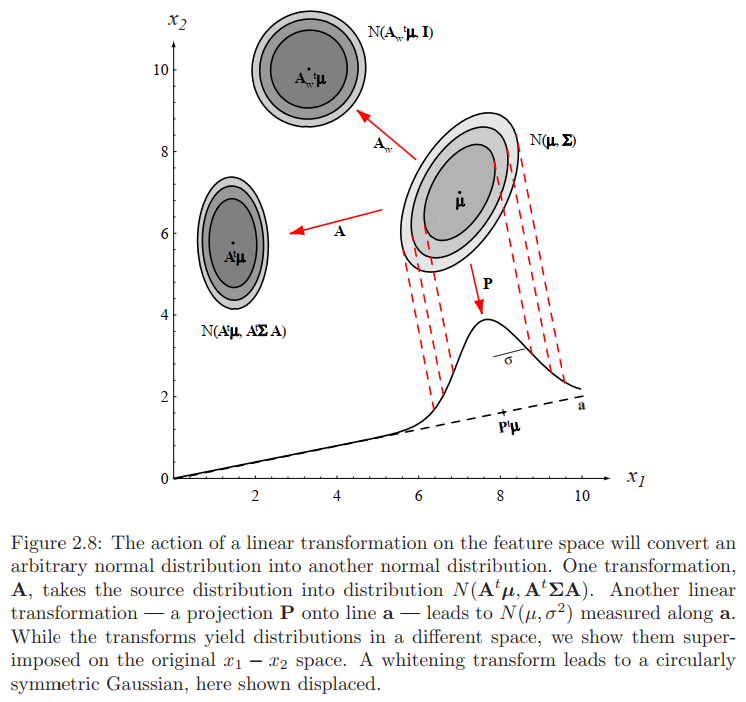
\includegraphics[width=0.8\linewidth]{fig/covariance_matrix.png}
\end{figure}

某个分布的协方差矩阵与单位阵$I$成比例,若定义矩阵$\Phi$,其列向量是$\Sigma$的正交本征向量,$\Lambda$为与相应本征值对应的对角矩阵,变换
\[A_w=\Phi\Lambda^{-1/2}\]
将使变换后的分布的协方差矩阵成为\textbf{单位阵}\footnote{这种表示方法是$\Cov{A_w^\T}=I$},此变换称为白化变换。

从$\vx$到$\vmu$的平方马氏(Mahalanobis)距离定义为(即正态分布中的指数部分)
\[r^2=(\vx-\vmu)^\T\Sigma^{-1}(\vx-\vmu)\]
可以证明与一Mahalanobis距离$r$对应的超椭球体体积为
\[V=V_d|\Sigma|^{1/2}r^d\]
其中$V_d$是一个$d$维单位超球体的体积
\[V_d=\begin{cases}
\pi^{d/2}/(d/2)! & d\text{为偶数}\\
2^d\pi^{(d-1)/2}\lrp{\frac{d-1}{2}}!/d! & d\text{为奇数}
\end{cases}\]
因此对于一给定维数,样本的离散程度直接随$|\Sigma|^{1/2}$而变化。

最小误差概率分类可用判别函数获得
\[g_i(\vx)=\ln p(\vx\mid\omega_i)+\ln P(\omega_i)\]
如果$p(\vx\mid\omega_i)\thicksim N(\vmu,\Sigma)$,则可以求得
\[g_i(\vx)=-\frac{1}{2}(\vx-\vmu)^\T\Sigma_i^{-1}(\vx-\vmu_i)-\frac{d}{2}\ln 2\pi-\frac{1}{2}\ln|\Sigma_i|+\ln P(\omega_i)\]